% 2026-10-23：按学习复现、探索尝试、优化验证、迭代调试、整板尝试重组。
\documentclass[stage2,fontset=fandol]{ydzjreport}
\usepackage{subcaption,longtable}

\stagetwosetup
{第 4 个逻辑月 · 迭代与调试}
{冯旭东、陈思文、张昊洋}
{复合微通道分区冷却}
{【待确认】逻辑月 4 对应的自然月}
{小块分界线；结构复杂性；Bi；扰流柱数量；XGBoost 待开展}
{探究不同热流密度下小块选择的适用边界，围绕 Bi 与扰流柱数量迭代理论，并准备基于翼型参数分组的 XGBoost 尝试。}
\pagestyle{empty}   % 去掉页眉与页脚（含页码）
\RemoveFromHook{enddocument}[ydzjreport] % 去掉末页的作者与格式规范收尾说明


\newlabel{eq:bi}{{1}{1}{Bi 验证思路与小块理论边界}{equation.2.1}{}}
\begin{document}
\section*{逻辑月4\_迭代与调试：图表附件}
本附件图表编号与对应提交正文及完整报告一致。\par\clearpage
\setcounter{table}{0}
\begin{table}[H]\centering
\caption{本月工作与材料状态}\label{tab:tasks}
\begin{tabularx}{\textwidth}{@{}Y Y Y@{}}
\toprule
\rowcolor{ydzjlight} 工作 & 状态 & 依据或缺口 \\
\midrule
小块适用分界线 & 研究问题已明确 & 尚缺统一约束下的扫描数据和交界热流密度 \\
复杂性与性能关系 & 已有探索依据 & 现有记录可提示问题，尚不能给出通用排序 \\
Bi 验证 & 待补依据 & 需给出特征尺度、物性、换热系数及计算结果 \\
扰流柱数量影响 & 研究重点已明确 & 需数量对照和换热、水力指标支持定量判断 \\
翼型 XGBoost & 尚未开展 & 待月三分组数据补齐后训练和测试 \\
\bottomrule\end{tabularx}\end{table}
\clearpage
\setcounter{figure}{0}
\begin{figure}[htbp]
\centering
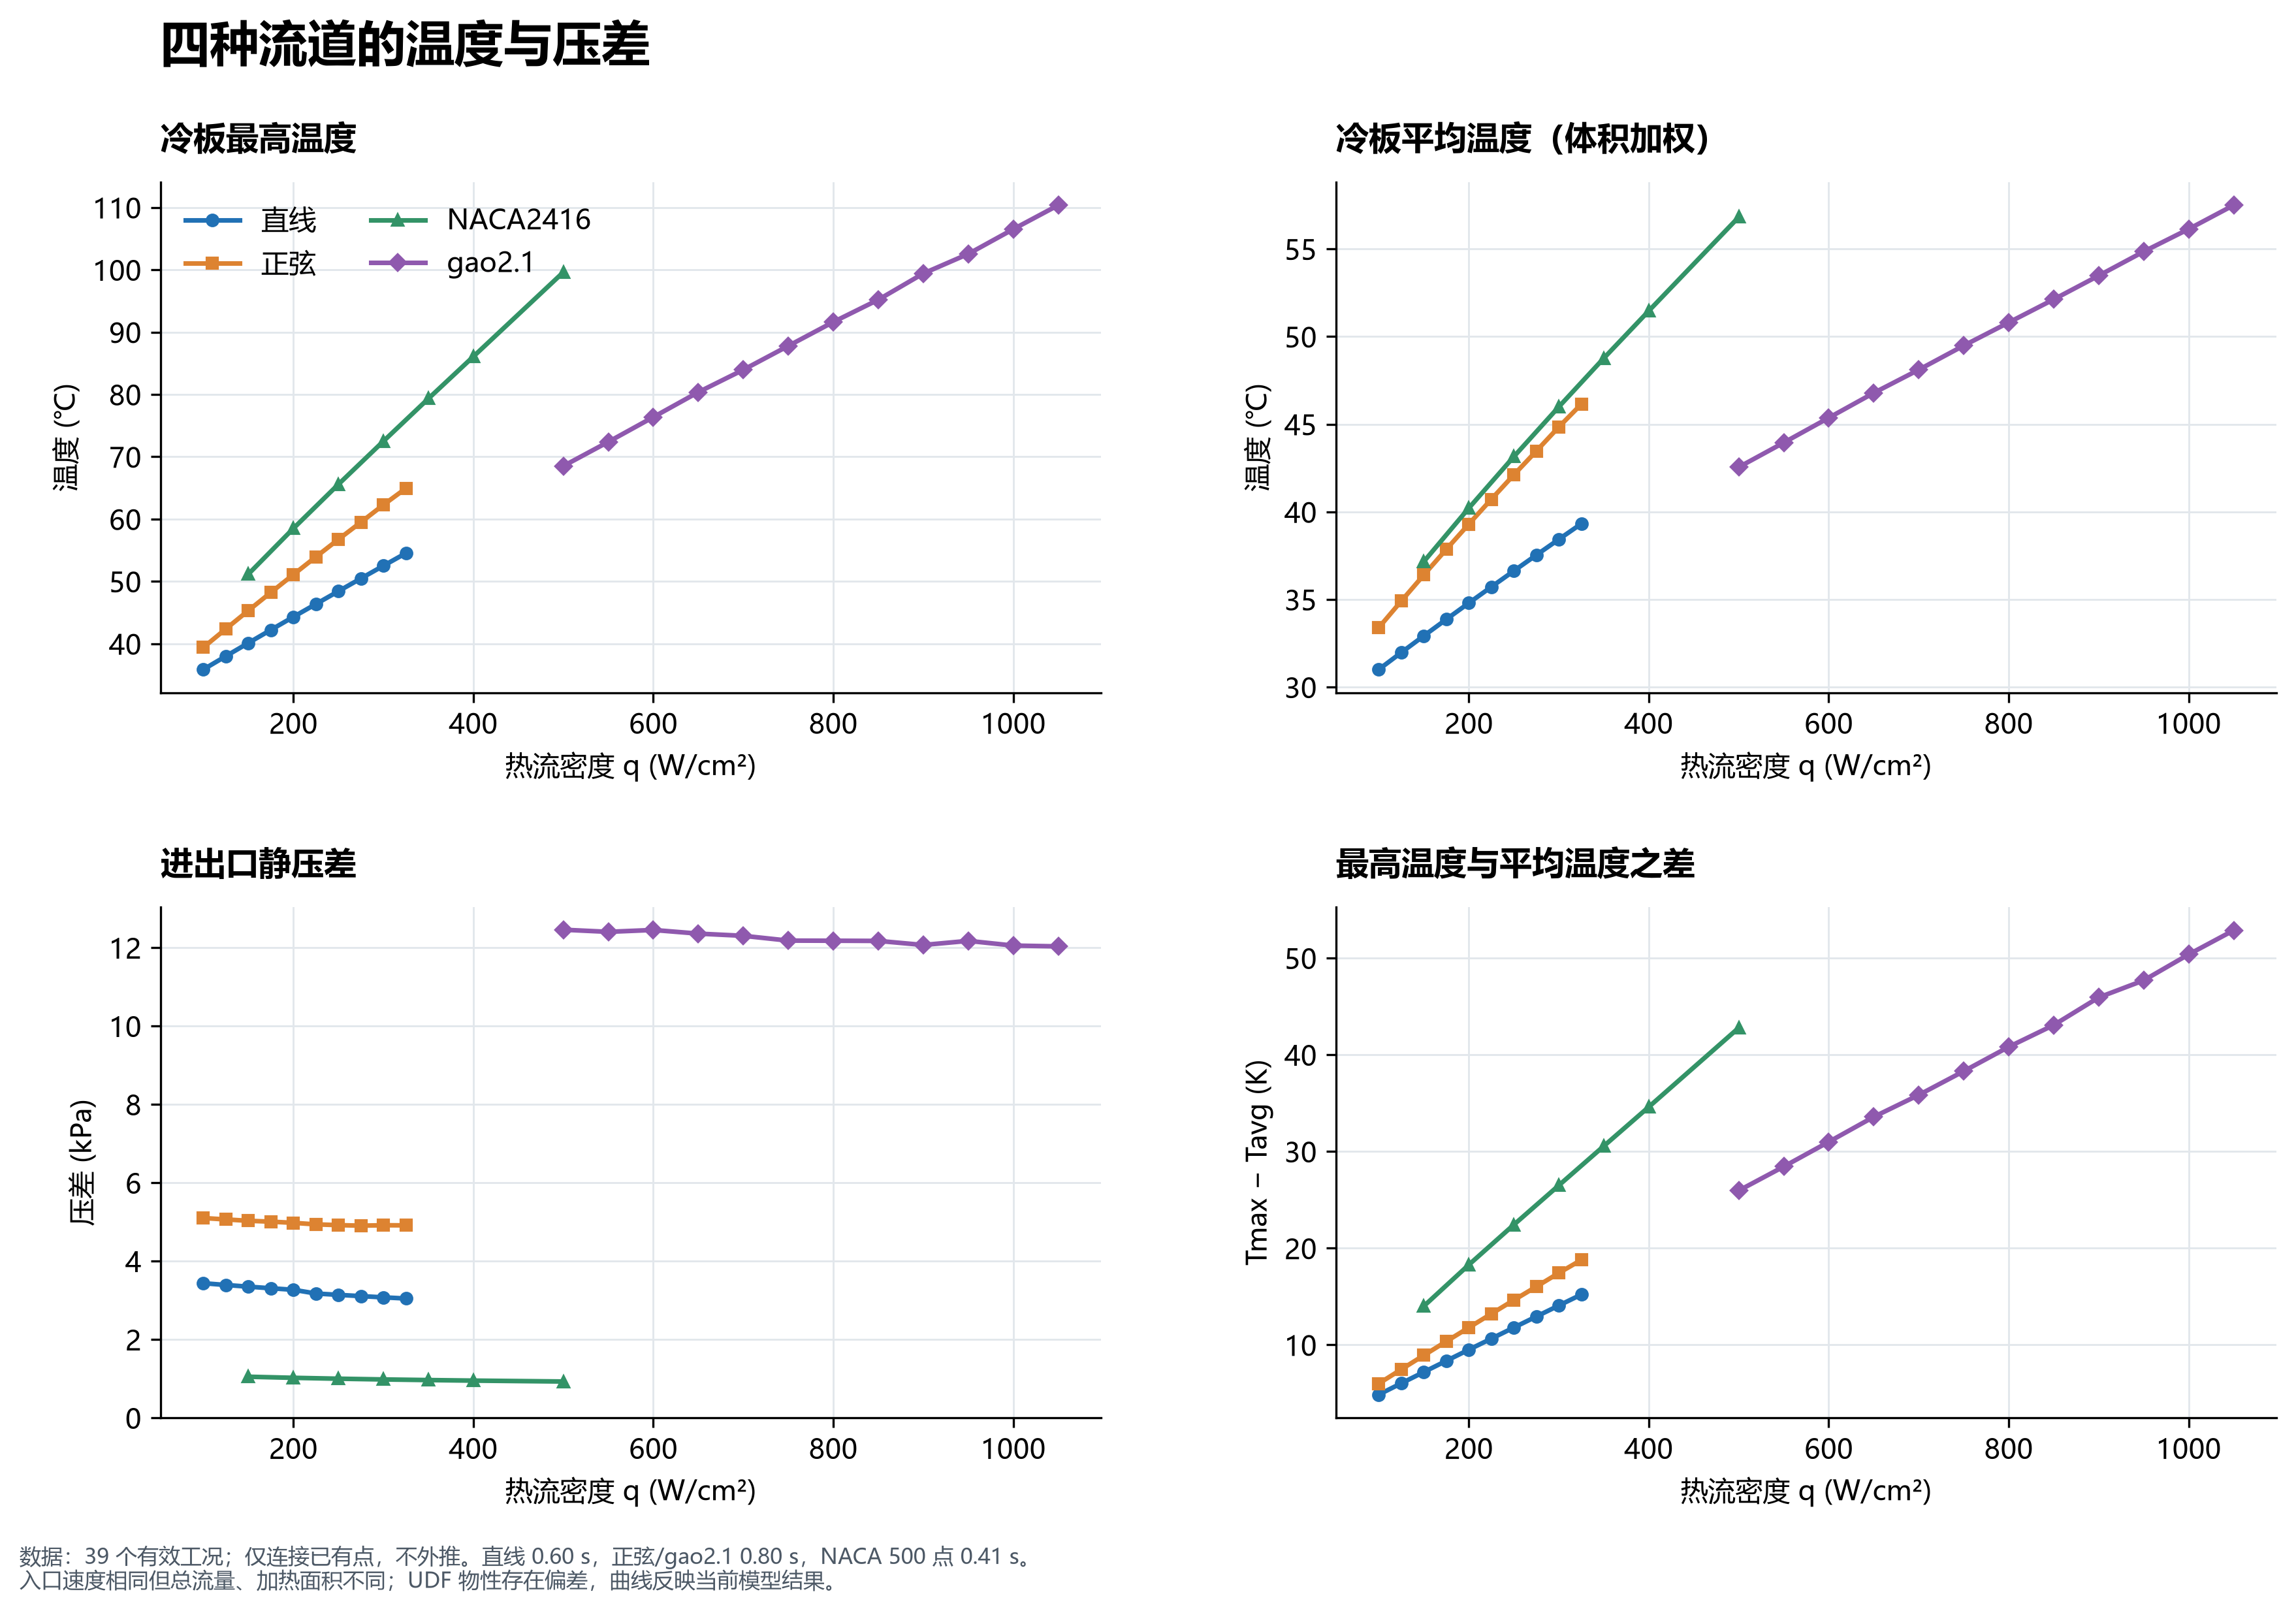
\includegraphics[width=\textwidth]{../../figs/30_四流道总览.png}
\caption{四种流道的最高温度、体积平均温度、进出口静压差与峰值—平均温差随热流密度的变化。仅连接已算点，不插值外推；gao2.1 从 500 W/cm$^2$ 起，直线与正弦止于 325 W/cm$^2$。}
\label{fig:month4-trend}
\end{figure}
\clearpage
\setcounter{table}{1}
\begin{table}[H]\centering\small
\caption{四种流道的工况与几何核对}\label{tab:month4-conditions}
\begin{tabularx}{\textwidth}{@{}l c c c c c@{}}
\toprule
\rowcolor{ydzjlight} 流道 & $q$ 范围 & 总入口面积 & 流量 & 加热面积 & 保存时刻 \\
 & / (W/cm$^2$) & / mm$^2$ & / (L/min) & / cm$^2$ & / s \\
\midrule
直线     & 100--325  & 8.00 & 0.96 & 0.1050 & 0.60 \\
正弦     & 100--325  & 6.00 & 0.72 & 0.1225 & 0.80 \\
NACA2416 & 150--500  & 8.00 & 0.96 & 0.1225 & 0.80\\
gao2.1   & 500--1050 & 4.50 & 0.54 & 0.1225 & 0.80 \\
\bottomrule
\end{tabularx}
\end{table}
\clearpage
\setcounter{figure}{1}
\begin{figure}[htbp]
\centering
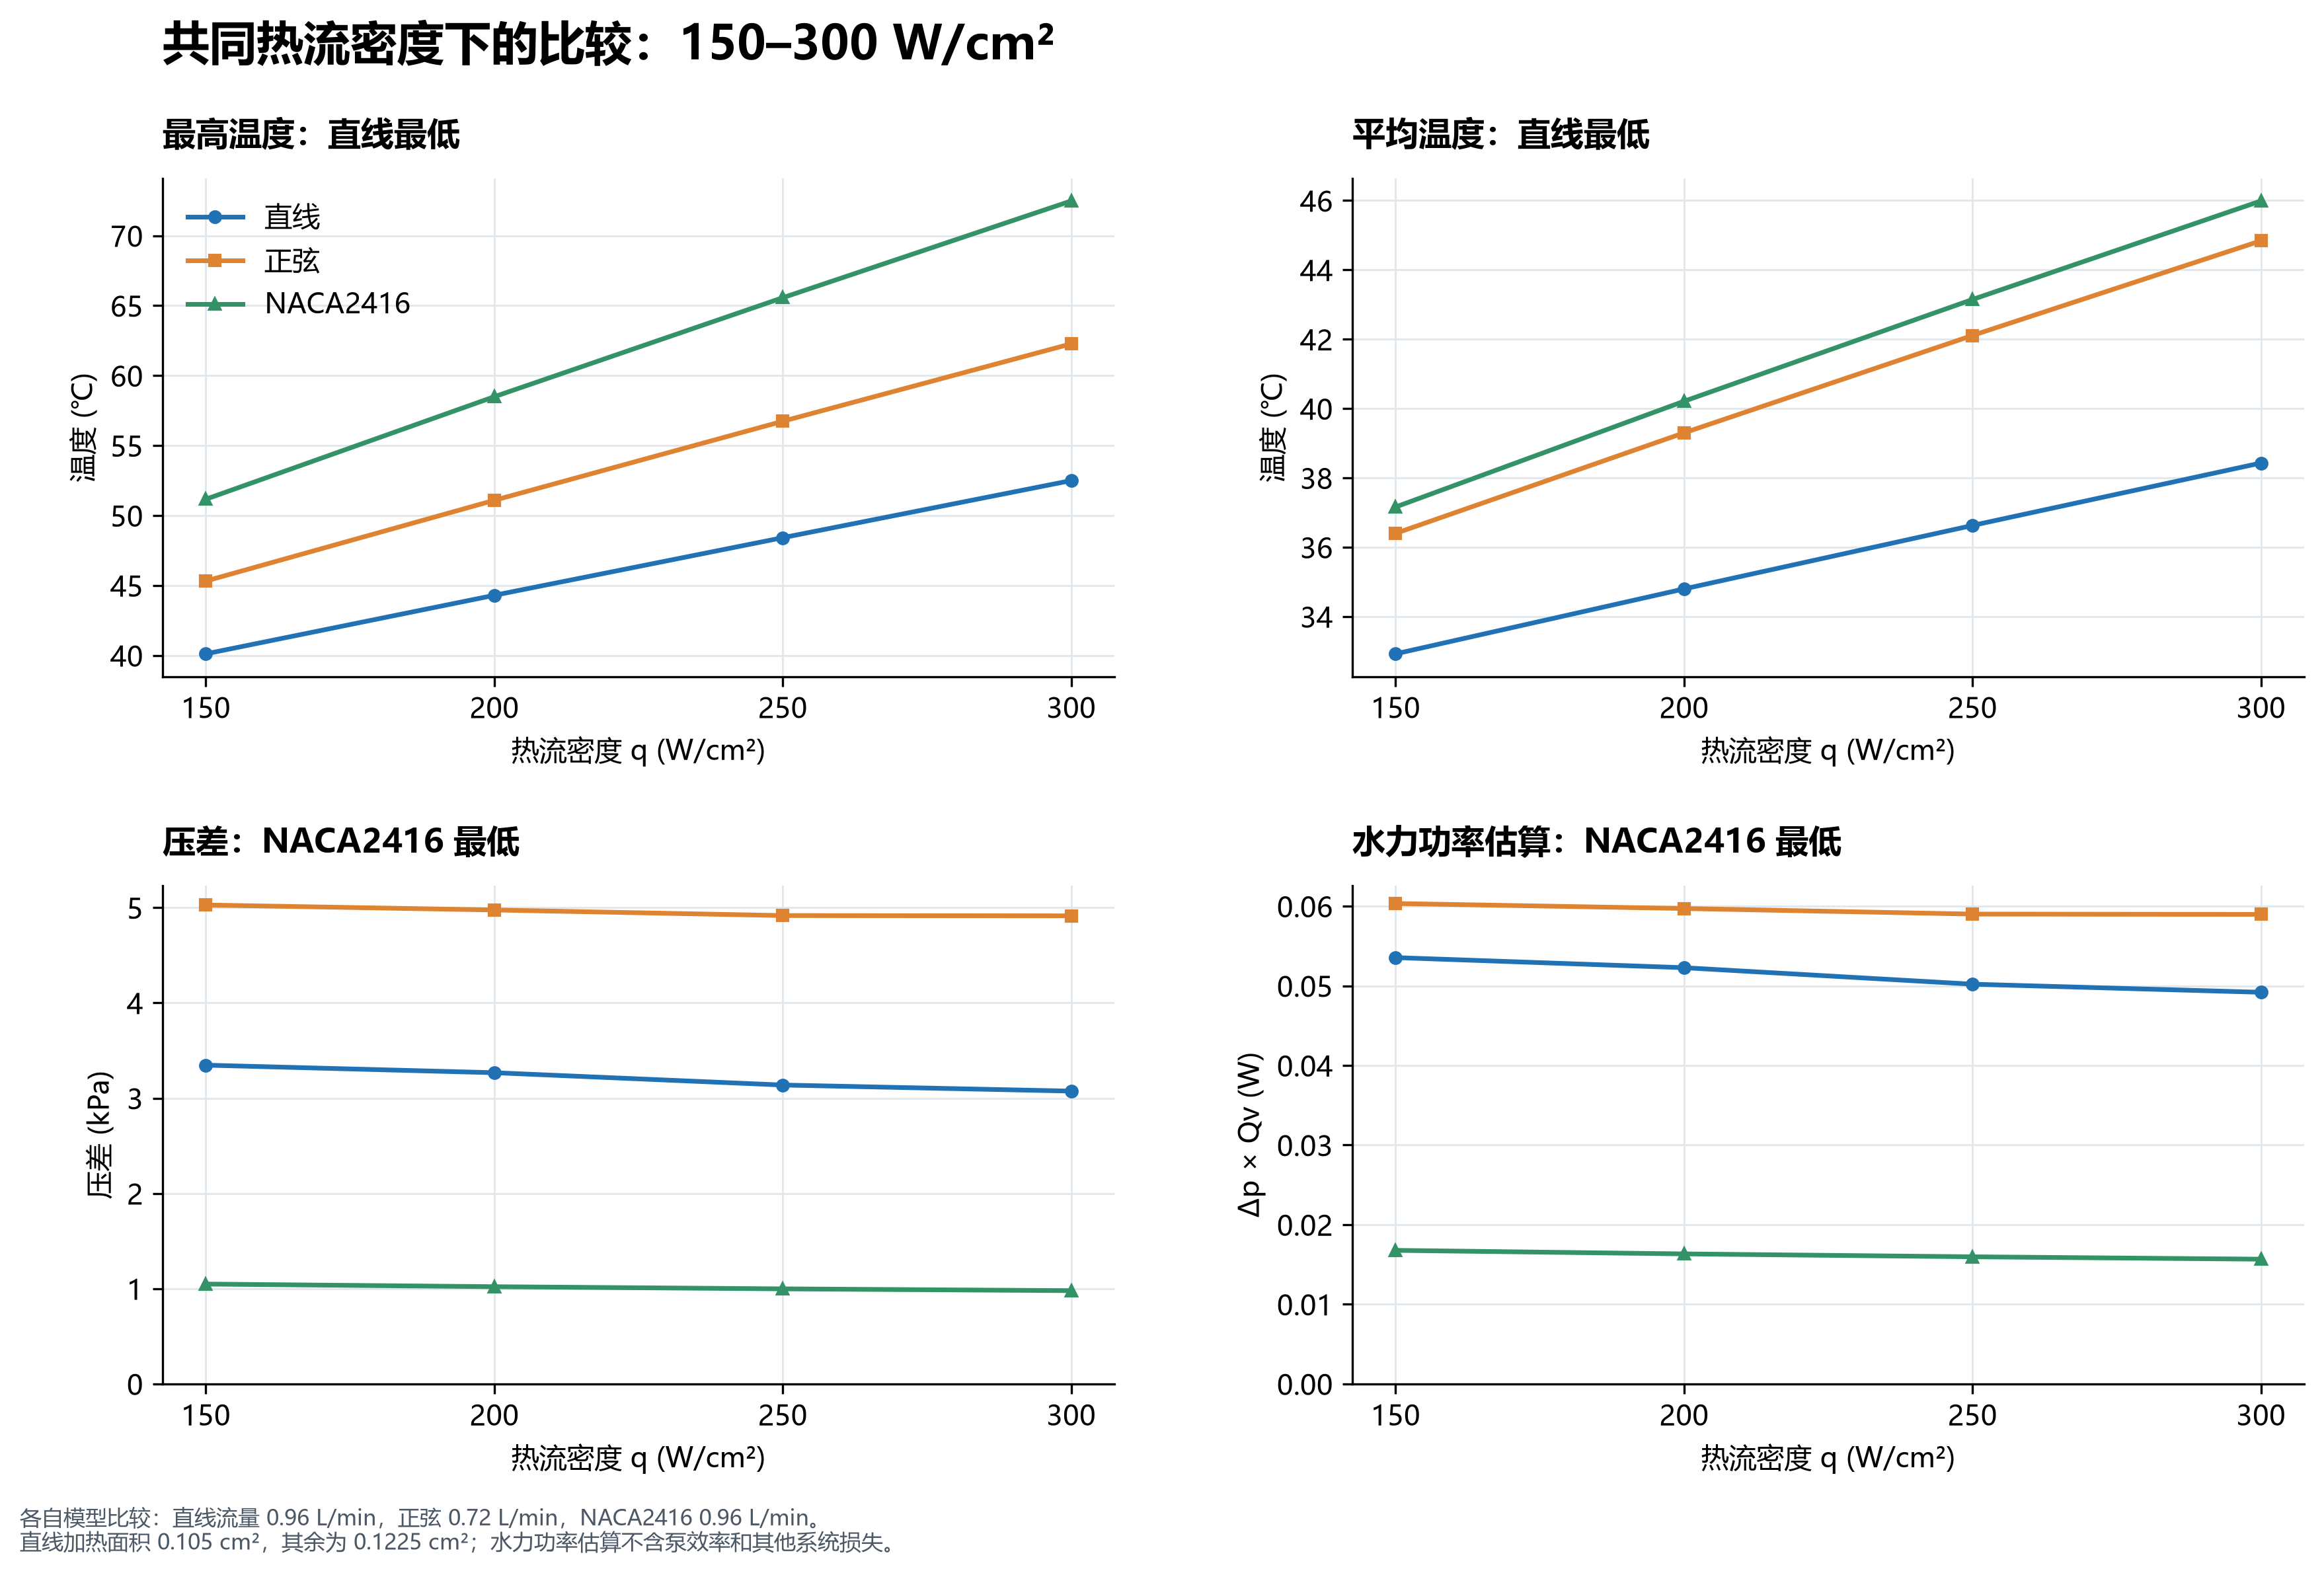
\includegraphics[width=\textwidth]{../../figs/31_共同热流密度比较.png}
\caption{150、200、250、300 W/cm$^2$ 四个共同数据点上的比较：最高温度、体积平均温度、压差与水力功率估算。}
\label{fig:month4-common}
\end{figure}
\clearpage
\setcounter{table}{2}
\begin{table}[H]\centering
\caption{四种流道的适用区间与依据}\label{tab:month4-advice}
\begin{tabularx}{\textwidth}{@{}l Y Y@{}}
\toprule
\rowcolor{ydzjlight} 流道 & 适用区间与定位 & 数据依据 \\
\midrule
直线 & 中低热流密度，温度优先 & 100--325 W/cm$^2$；共同区间内最高温度、平均温度均最低，压差与水力功率低于正弦 \\
正弦 & 中低热流密度，与直线同档 & 100--325 W/cm$^2$；温度略高于直线、压差与水力功率略高，仍低于 NACA2416 的温度水平 \\
NACA2416 & 中低热流密度，压降优先 & 150--500 W/cm$^2$；共同区间内压差与水力功率最低，为直线的 31.8\%、正弦的 19.9\%，300 W/cm$^2$ 时最高温度 72.5 $^\circ$C \\
gao2.1 & 高热流密度 & 500--1050 W/cm$^2$；500 点最高温度 68.50 $^\circ$C，1050 点 110.36 $^\circ$C，是唯一覆盖 1000 W/cm$^2$ 以上的方案 \\
\bottomrule
\end{tabularx}
\end{table}
\clearpage
\setcounter{figure}{2}
\begin{figure}[htbp]
\centering
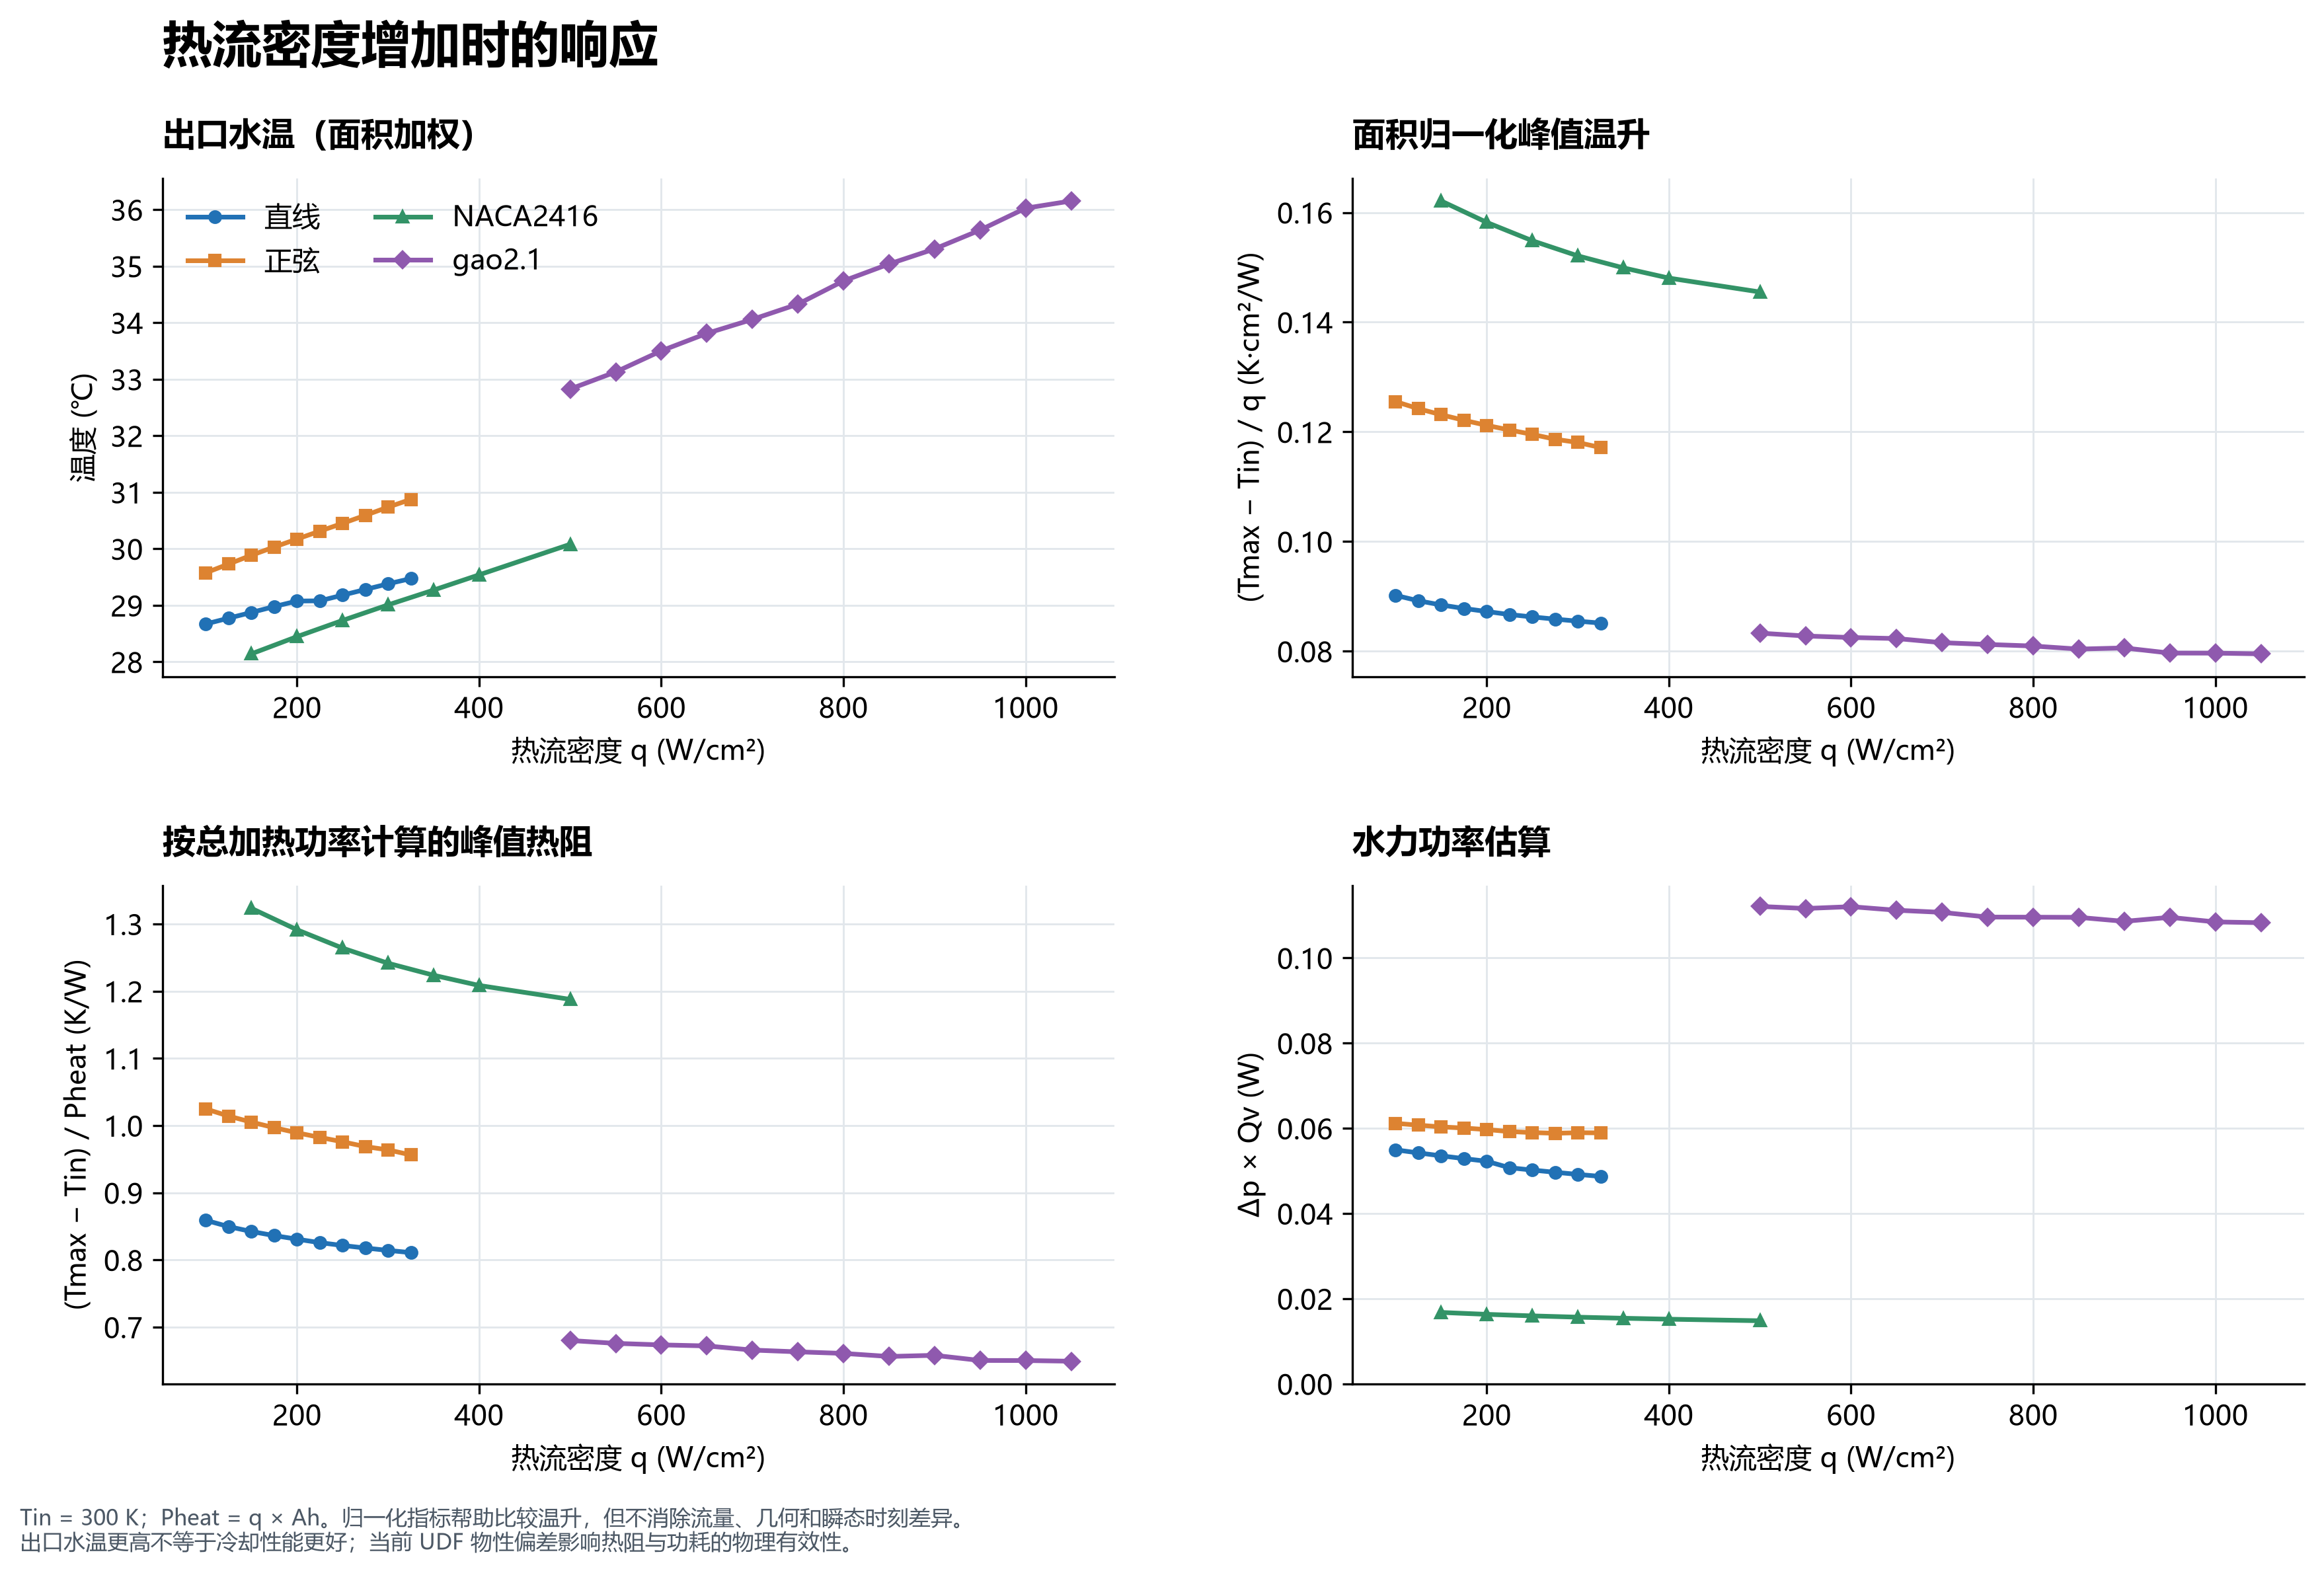
\includegraphics[width=\textwidth]{../../figs/32_归一化指标与水力代价.png}
\caption{出口水温、面积归一化峰值温升、按总加热功率计算的峰值热阻与水力功率估算随热流密度的变化。$R''_{\max}=(T_{\max}-T_{\mathrm{in}})/q$，$R_{\max}=(T_{\max}-T_{\mathrm{in}})/(qA_h)$，$P_{\mathrm{hyd}}=\Delta p\,Q_v$。}
\label{fig:month4-normalized}
\end{figure}
\clearpage
\setcounter{figure}{3}
\begin{figure}[htbp]
\centering
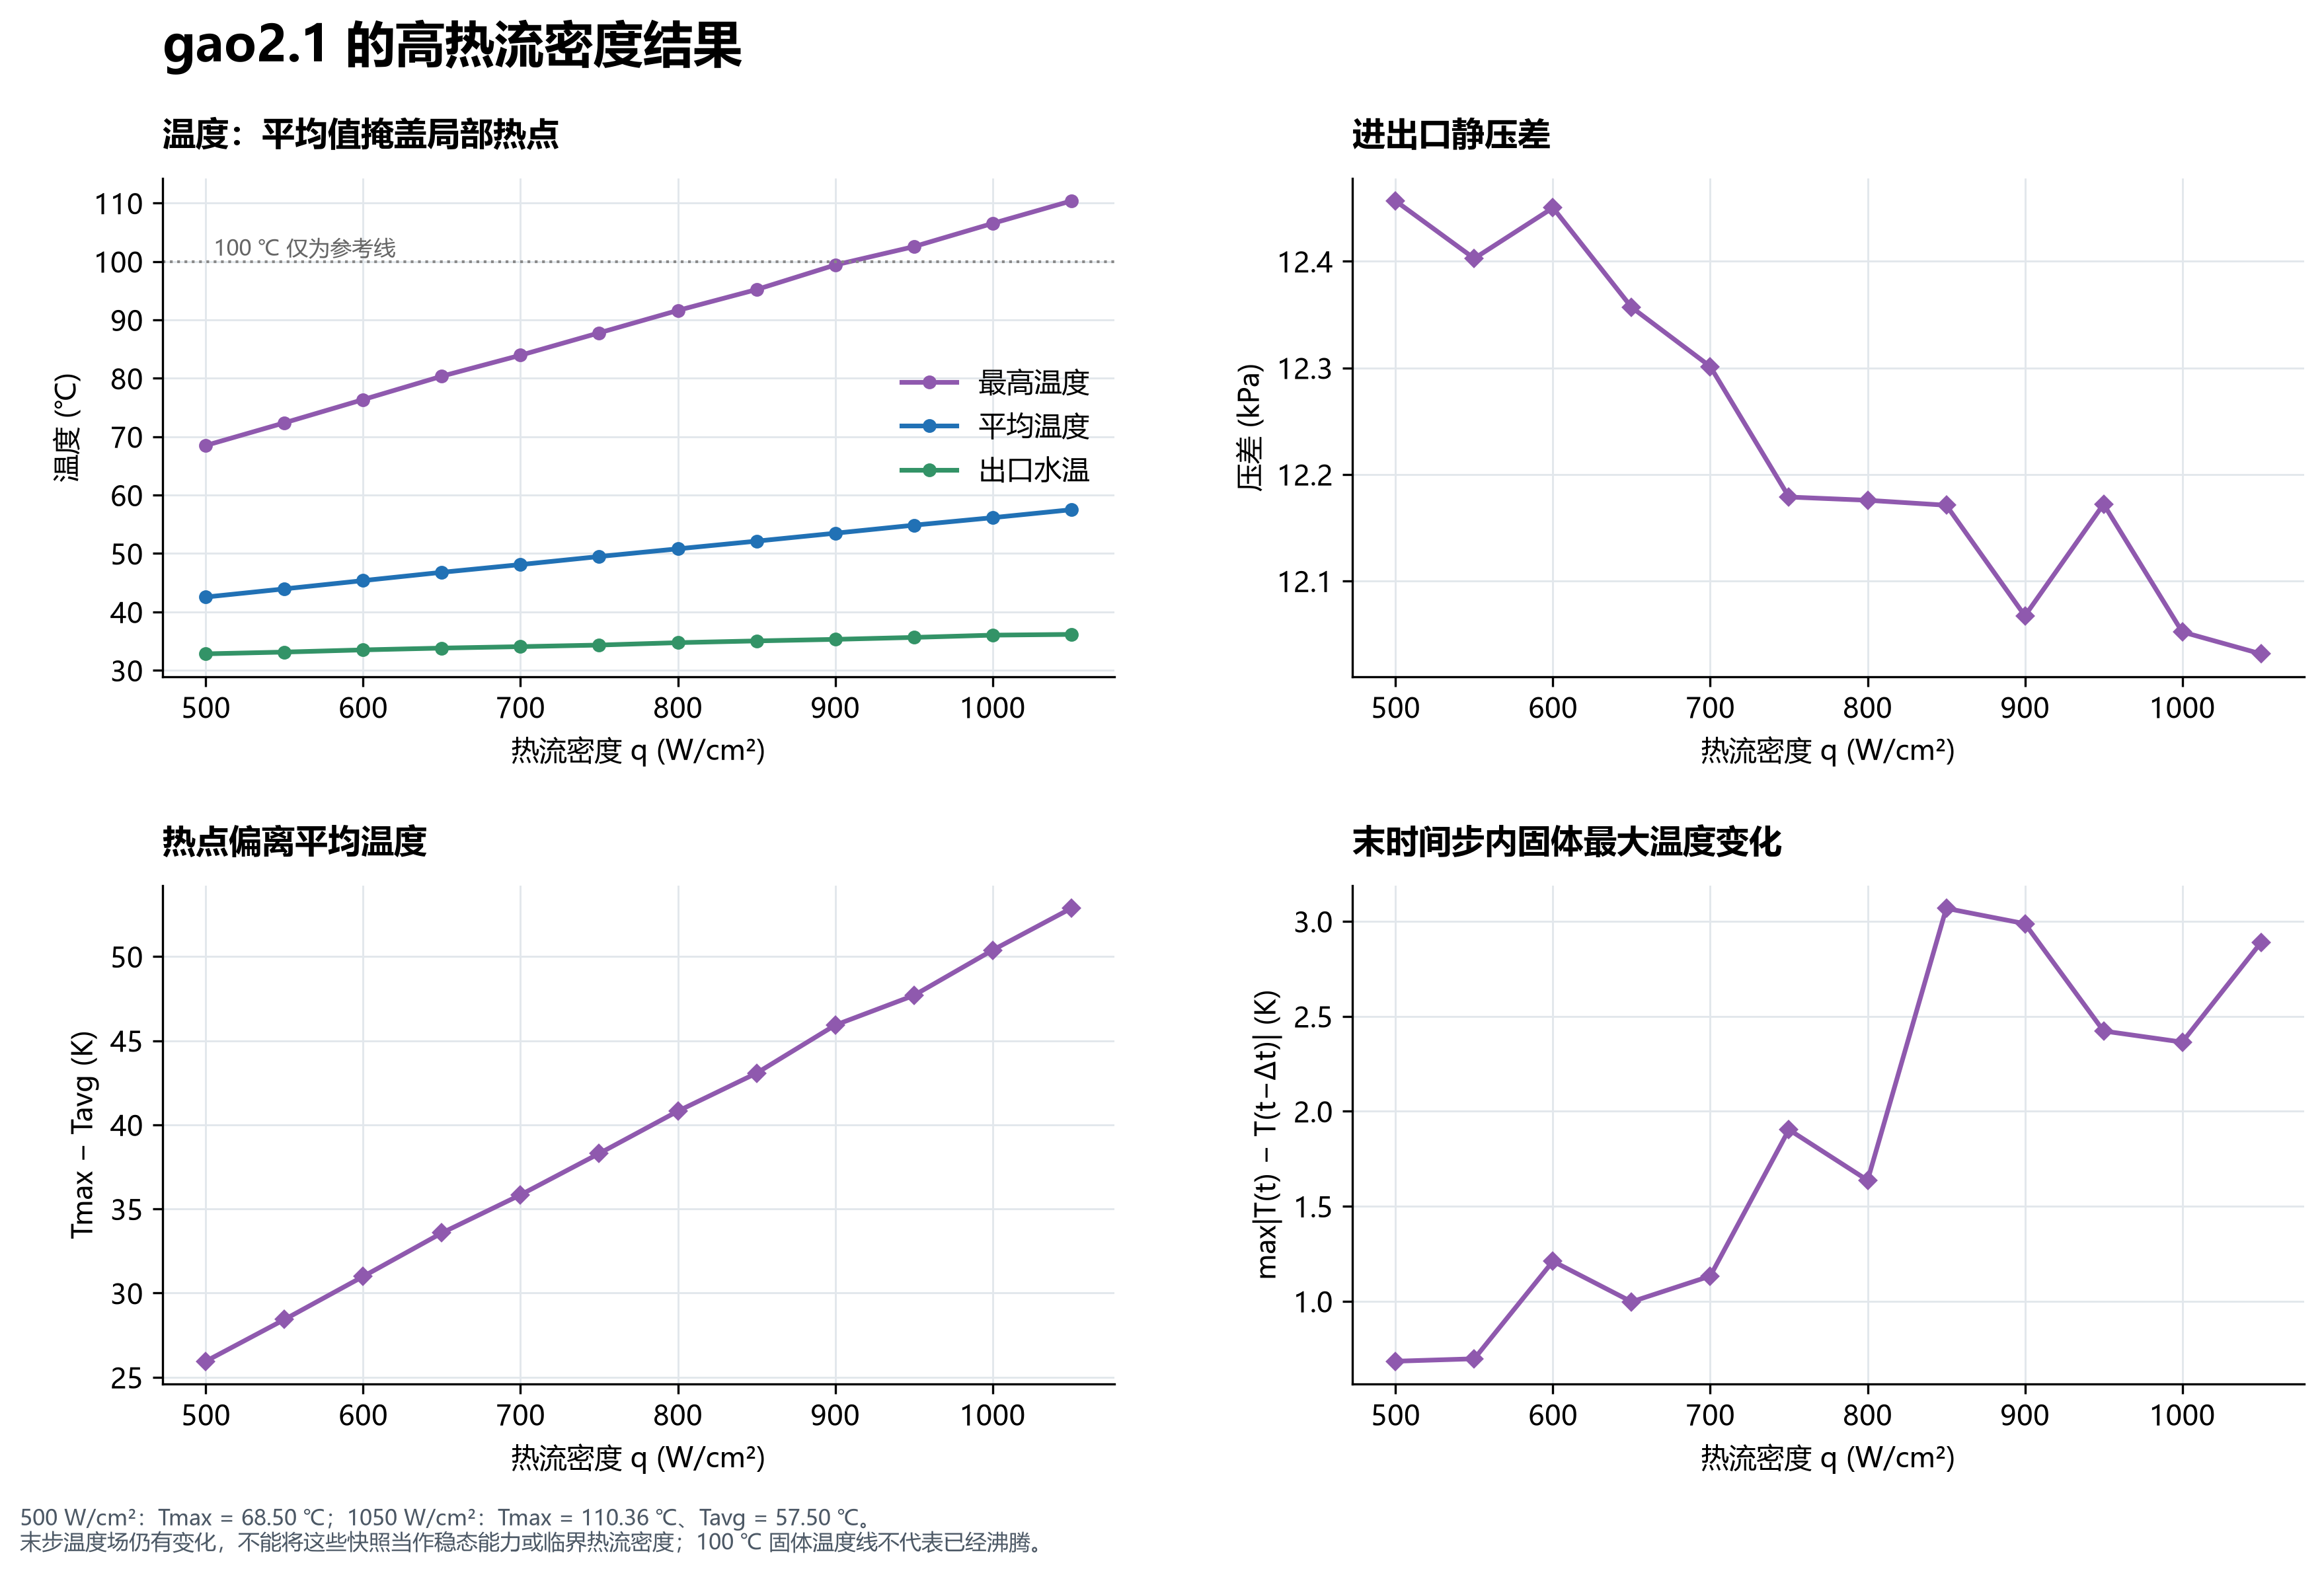
\includegraphics[width=\textwidth]{../../figs/33_gao2.1高热流密度.png}
\caption{gao2.1 在 500--1050 W/cm$^2$ 区间的温度、压差与末时间步温度变化。最高温度由 500 点的 68.50 $^\circ$C 升至 1050 点的 110.36 $^\circ$C，1050 点体积平均温度仅 57.50 $^\circ$C。}
\label{fig:month4-gao}
\end{figure}
\clearpage
\setcounter{figure}{4}
\begin{figure}[htbp]
\centering
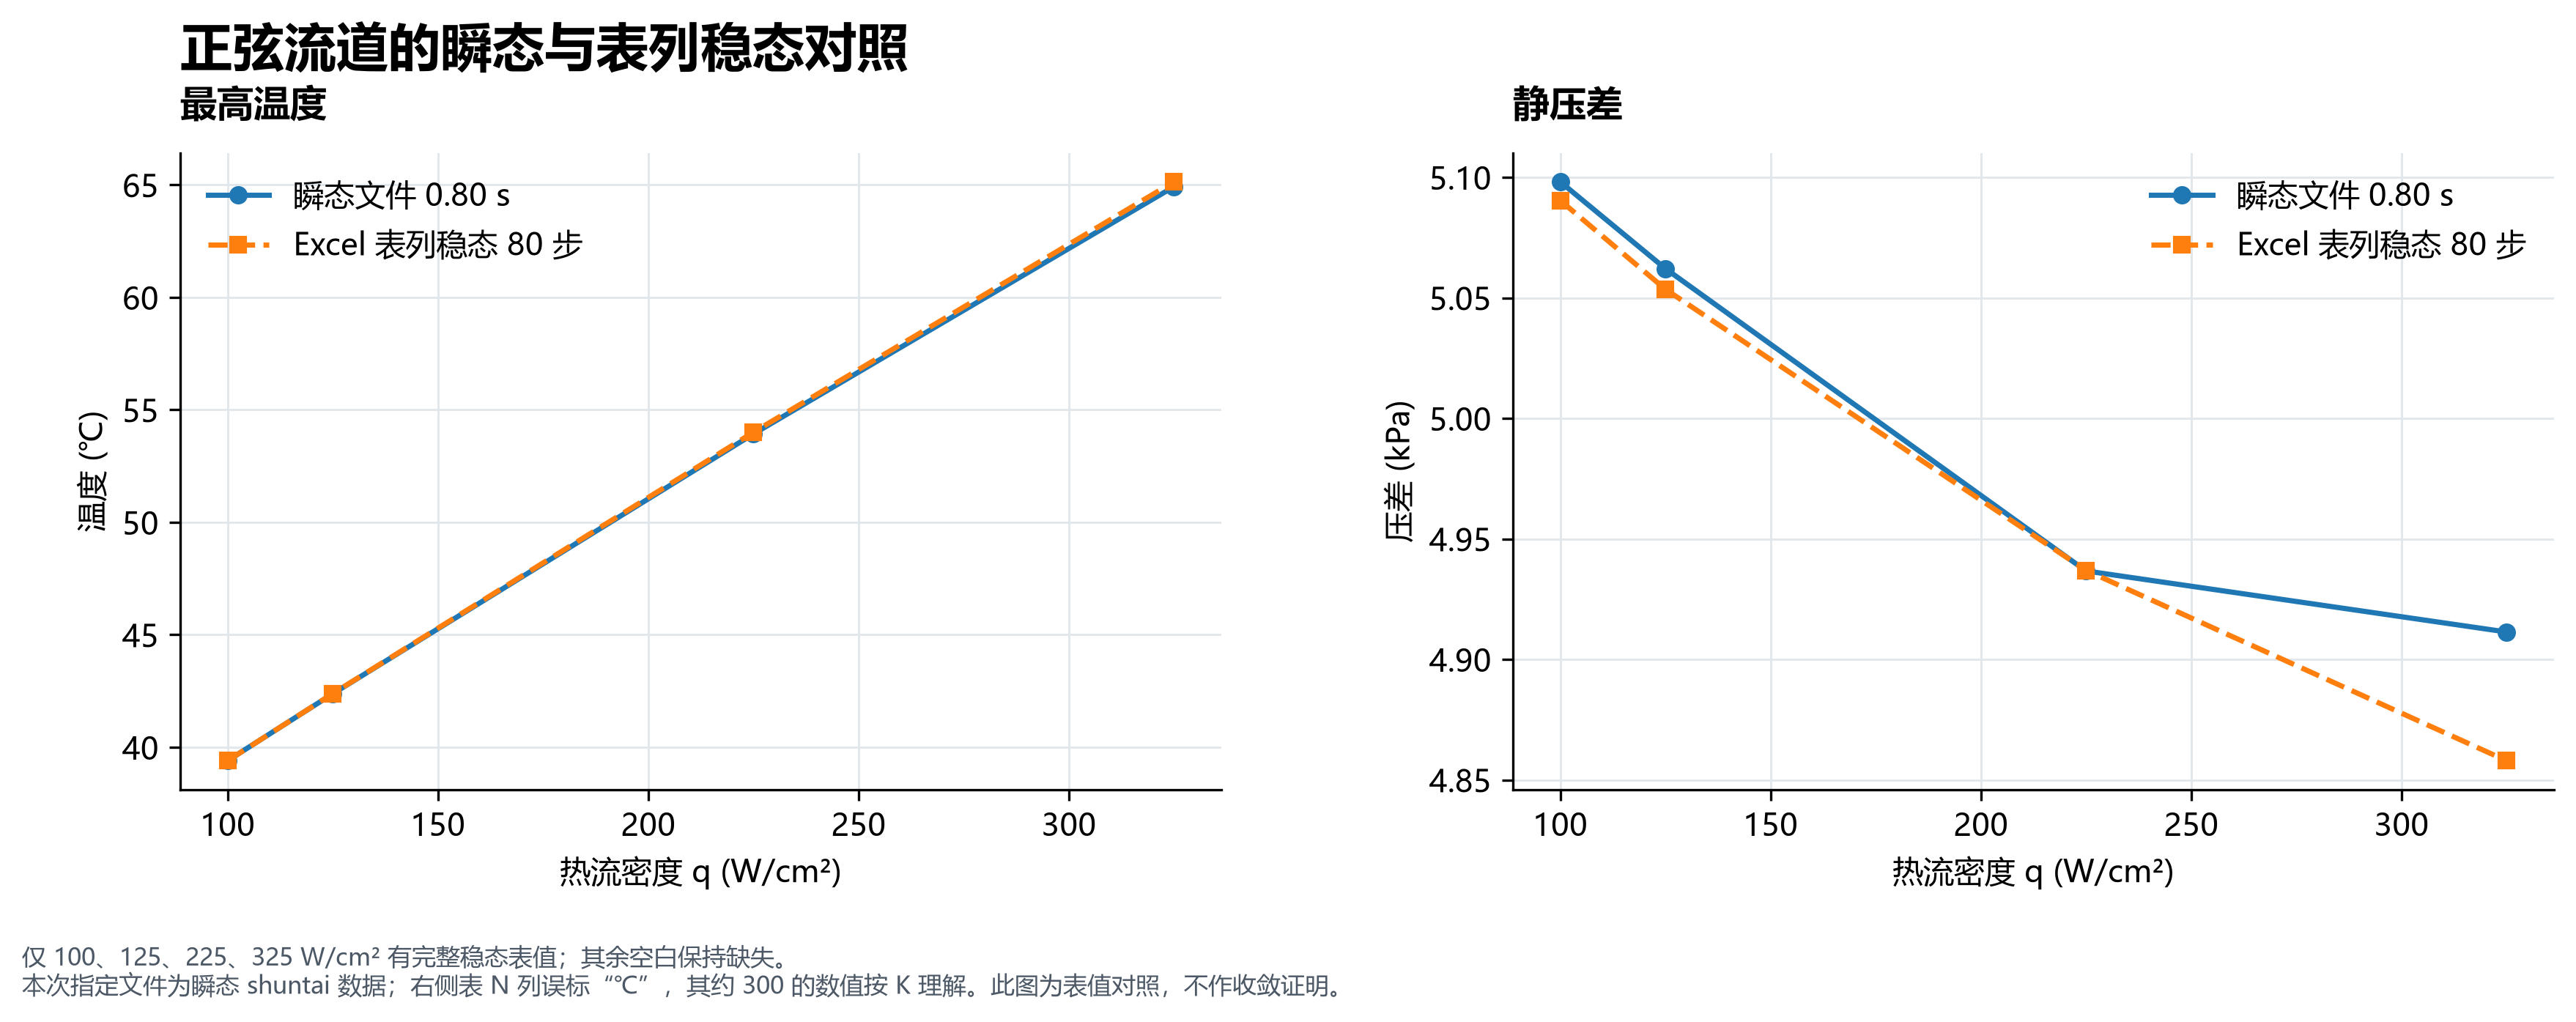
\includegraphics[width=\textwidth]{../../figs/35_正弦稳态对照.png}
\caption{正弦流道瞬态文件（0.80 s）与表列稳态结果的对照：最高温度与静压差。}
\label{fig:month4-sin-steady}
\end{figure}
\clearpage
\setcounter{table}{3}
\begin{table}[H]\centering
\caption{后续工作及所需产出}\label{tab:plan}
\begin{tabularx}{\textwidth}{@{}Y Y Y@{}}
\toprule
\rowcolor{ydzjlight} 工作 & 状态 & 依据或缺口 \\
\midrule
补充理论迭代证据 & 分界线、Bi 与数量对照 & 持续补充 \\
补齐分组并尝试代理模型 & 训练记录及独立测试 & 具备数据后 \\
将局部研究接入整板 & 候选布局、连接和供液条件 & 逻辑月五 \\
\bottomrule\end{tabularx}\end{table}
\clearpage
\begin{thebibliography}{9}
\bibitem{proposal} 大创项目申报书：研究内容与实施方案. 2026.
\bibitem{udf} 项目组. water\_properties\_refprop\_fit.c：液态水物性拟合与 Fluent UDF 源码. 项目计算资料, 2026.
\bibitem{data} 四种流道数据与折线图. 项目计算资料, 2026.
\end{thebibliography}
\end{document}
